\documentclass[12pt]{article}

% Ustawienia strony
\usepackage{lipsum}
\usepackage[margin=1.5cm]{geometry}
\usepackage{graphicx}
\usepackage{enumitem}
\usepackage{siunitx}
\usepackage{amsmath}
\usepackage{cancel}
\usepackage{makecell}
\usepackage{mathtools}
\usepackage{floatrow}
\usepackage{caption}
\usepackage[T1]{fontenc}
\usepackage{fancyvrb}
\usepackage[ngerman]{babel} %Deutsche Sprachunterstützung
\usepackage{subcaption}
\usepackage{graphicx}
\usepackage{blindtext}
\usepackage{hyperref}
\usepackage[dvipsnames]{xcolor}

\hypersetup{
	colorlinks=true,
	linkcolor=blue,
	filecolor=magenta,      
	urlcolor=cyan,
	pdfpagemode=FullScreen,
}

\urlstyle{same}

\fvset{tabsize=4}
\setlist{leftmargin=15pt,labelindent=15pt}
\setlist[enumerate]{noitemsep,wide=0pt, leftmargin=*}
{\setlength{\parindent}{0pt}
	
	% Ustawienia stopki
	\usepackage{lastpage}
	\usepackage{fancyhdr}
	\pagestyle{fancy}
	\fancyhf{} % sets both header and footer to nothing
	\renewcommand{\headrulewidth}{0pt}
	\cfoot{\thepage\ z \pageref*{LastPage}}
	
	\begin{document}
		
		\section*{Podstawowe dane}
		\begin{figure}[htp]
			\begin{minipage}[t]{0.3\textwidth}
				\textbf{Imie i nazwisko} \\
				\textbf{Data} \\
				\textbf{Tytuł} \\
				\textbf{Numer ćwiczenia}
			\end{minipage}%
			\begin{minipage}[t]{0.6\textwidth}
				Robert Mesek \\
				14.12.2023 \\
				Algorytmy geometryczne \\
				4
			\end{minipage}%
		\end{figure}
		
		\section*{Dane techniczne}
		\begin{figure}[htp]
			\begin{minipage}[t]{0.3\textwidth}
				\textbf{Procesor} \\
				\textbf{Język} \\
				\textbf{Biblioteki} \\
				\textbf{System operacyjny} \\
				\textbf{Środowisko}
				
			\end{minipage}%
			\begin{minipage}[t]{0.7\textwidth}
				Intel i7-1165G7 x86\_64 \\
				Python 3.11.5 \\
				NumPy 1.26.0, sortedcontainers 2.4.0, Matplotlib 3.8.0, seaborn 0.13.0 \\
				WSL Ubuntu 22.04 (MS Windows 10 22H2) \\
				conda 23.5.2
			\end{minipage}%
		\end{figure}
		
		\subsection*{Cel ćwiczenia}
		\begin{figure}[htp]
			\begin{minipage}[t]{0.5\textwidth}
				\vspace{1em}
				
				Celem ćwiczenia jest:
				
				- sprawdzanie czy dowolne odcinki się przecinają
				
				- znalezienie wszystkich przecięć odcinków
				
			\end{minipage}%
			\hfill
			\begin{minipage}[t]{0.5\textwidth}
				\centering
				\vspace{0pt}
				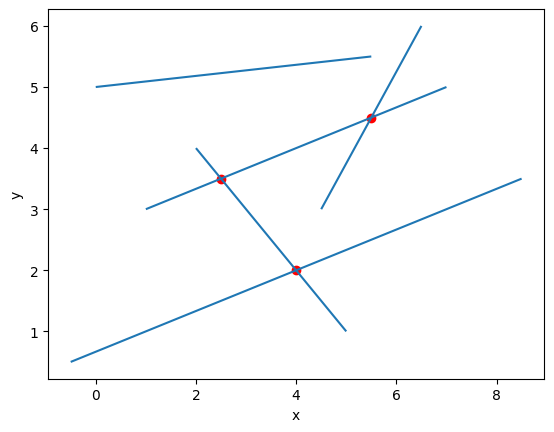
\includegraphics[width=1\linewidth]{images/przyklad.png}
				
				\verb|Rys. 1|: przecinające się odcinki
			\end{minipage}%
			\hspace*{\fill}
		\end{figure}
		
		\subsection*{Zastosowania triangulacji} 
		Algorytm wyznaczania przecięć odcinków jest wykorzystywany w wielu gałęziach informatki. W robotyce podczas planowania ruchu robota, w grafice komputer, aby znaleźć nachodzące na siebie figury geometryczne, w rozwiązywaniu problemów algorytmicznych m.in. nakłania się map.
		
		\newpage
		
		\subsection*{Dodatkowe założenia przyjmowane w tym zadaniu}
		\begin{itemize}
			\item Żaden odcinek nie jest pionowy
			\item Dwa odcinki przecinają się w co najwyżej jednym punkcie
			\item Żadne trzy odcinki nie przecinają się w jednym punkcie
		\end{itemize}
		
		\begin{figure}[H]
			\centering
			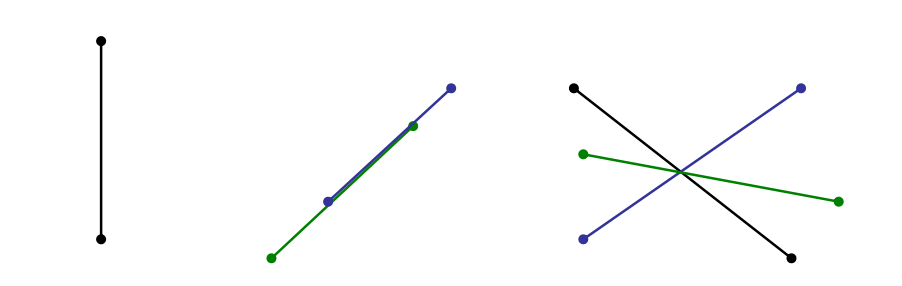
\includegraphics[width=0.7\linewidth]{images/wykluczone.png}
			
			\verb|Rys. 2: Wykluczone przypadki|
		\end{figure}
		
		\section*{Funkcje pomocnicze}
		\par Reprezentuje punkt
		\begin{Verbatim}
def generate_uniform_sections(max_x, max_y, n, eps_x=None):
	if eps_x is None:
		eps_x = 1 / 2 * (max_x - 0) / (2 * n)
	print(f"{eps_x=}")
	sections = []
	intervals = []
	def gen_x(min_x, max_x, intervals, eps):
		rand_x = np.random.uniform(min_x, max_x)
		while check_if_in_interval(rand_x, intervals):
			rand_x = np.random.uniform(min_x, max_x)
			intervals.append((rand_x - eps, rand_x + eps))
		return rand_x
	def check_if_in_interval(x, intervals):
		for start, end in intervals:
			if start < x < end:
				return True
		return False
	for _ in range(n):
		y1 = np.random.uniform(0, max_y)
		y2 = np.random.uniform(0, max_y)
		x1 = gen_x(0, max_x, intervals, eps_x)
		x2 = gen_x(0, max_x, intervals, eps_x)
		sections.append(((x1, y1), (x2, y2)))
	return sections
		\end{Verbatim}
		
\newpage
\section*{Rozkład losowo wygenerowanych punktów}
\par \verb|generate_uniform_sections(10, 10, 1000)|
\begin{figure}[htp]
	\begin{subfigure}[t]{.45\textwidth}
		\centering
		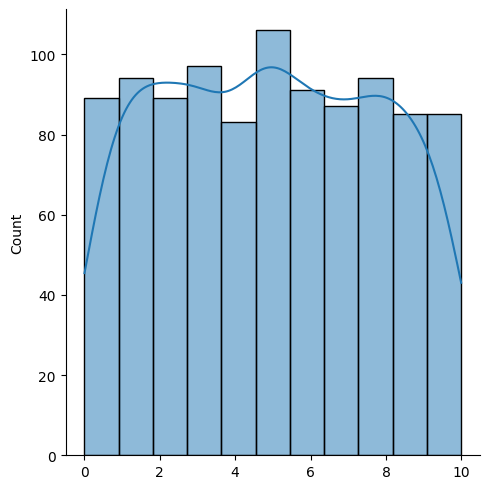
\includegraphics[width=\linewidth]{images/roz1.png}
		\caption*{Rys. 3: Rozkład x-ów początków odcinków}
	\end{subfigure}
	\hfill
	\begin{subfigure}[t]{.45\textwidth}
		\centering
		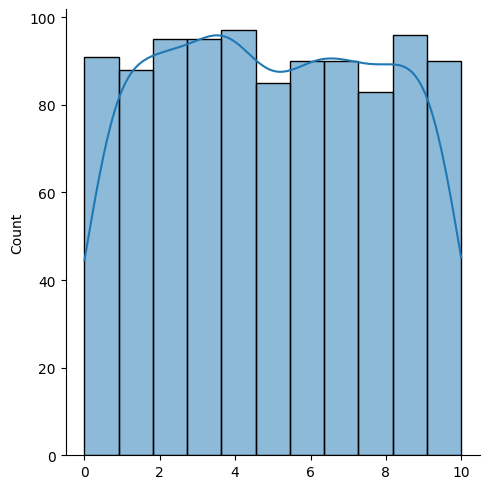
\includegraphics[width=\linewidth]{images/roz2.png}
		\caption*{Rys. 4: Rozkład x-ów końców odcinków}
	\end{subfigure}
\end{figure}

\begin{figure}[htp]
	\begin{subfigure}[t]{.45\textwidth}
		\centering
		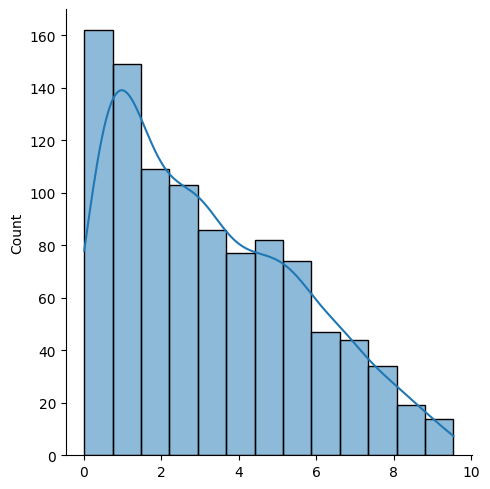
\includegraphics[width=\linewidth]{images/roz3.png}
		\caption*{Rys. 5: Rozkład modułu różnicy x-ów odcinków}
	\end{subfigure}
	\hfill
	\begin{subfigure}[t]{.45\textwidth}
		\centering
		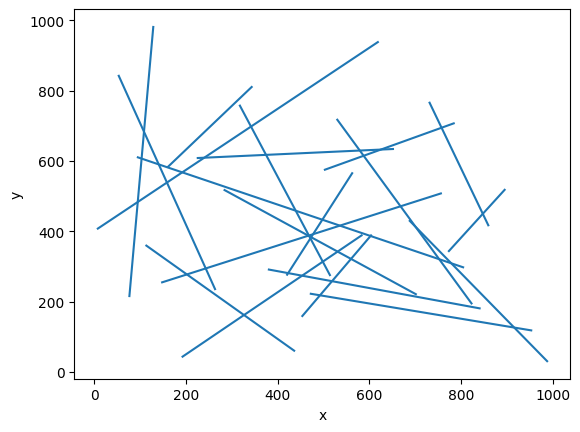
\includegraphics[width=\linewidth]{images/prz4.png}
		\caption*{Rys. 6: Losowe 20 odcinków}
	\end{subfigure}
\end{figure}


\newpage
\section*{Reprezentacja punktu i odcinka}
		\par Reprezentuje punkt
		\begin{Verbatim}
class Point:
	EPSILON = 10**-12
	def __init__(self, x, y, type, lines=None):
		self.x = x
		self.y = y
		# -1 - początek odcinka
		# 0 - przecięcie odcinków
		# 1 - koniec odcinka
		self.type = type
		if lines is None:
		self.lines = set()
		else:
		self.lines = lines
	def __repr__(self):
		return f"Point({self.x}, {self.y}, {self.type})"
	def distance(self, other):
		return ((other.x - self.x) ** 2 + (other.y - self.y) ** 2) ** 0.5
	def as_tuple(self):
		return (self.x, self.y)
	def __hash__(self) -> int:
		return hash((self.x, self.y, self.type))
	def __eq__(self, other: object) -> bool:
		if not isinstance(other, Point):
			return NotImplemented
		return self.distance(other) < self.EPSILON
	def __gt__(self, other: object) -> bool:
		if not isinstance(other, Point):
			return NotImplemented
		if abs(self.x - other.x) < self.EPSILON:
			return self.y > other.y
		return self.x > other.x
		\end{Verbatim}
		
		\subsection*{Metody klasy Line}
\begin{itemize}
	\item \verb|brush_x| aktualna współrzędna x-owa miotły
	\item \verb|get_y(x)| zwraca wartość funkcja dla danego \verb|x|
	\item Funkcja sprawdzająca równość prostych korzysta z unikalnego id, nadanego podczas tworzenia odcinków
	\item Funkcja porównania prostych porównuje odcinki względem wartości \verb|get_y(brush_x)| dla danego położenia miotły
\end{itemize}

		
\newpage
		\par Reprezentuje odcinek
\begin{Verbatim}
	class Line:
	brush_x = None
	
	def __init__(self, l_point: Point, r_point: Point, id):
	self.l_point = l_point
	self.r_point = r_point
	self.id = id
	
	def __repr__(self):
	return f"Line{self.id}({self.l_point}, {self.r_point})"
	
	def __hash__(self) -> int:
	return hash((self.l_point, self.r_point))
	
	def __eq__(self, other: object) -> bool:
	if not isinstance(other, Line):
	return NotImplemented
	return self.id == other.id
	# return self.l_point == other.l_point and self.r_point == other.r_point
	
	def __gt__(self, other: object) -> bool:
	if not isinstance(other, Line):
	return NotImplemented
	return self.get_y(self.brush_x) > other.get_y(other.brush_x)
	
	def get_y(self, x: float):
	a = (self.r_point.y - self.l_point.y) / (self.r_point.x - self.l_point.x)
	b = self.r_point.y - a * self.r_point.x
	return a * x + b
	
	def as_tuple(self):
	return ((self.l_point.x, self.l_point.y), (self.r_point.x, self.r_point.y))
\end{Verbatim}

\subsection*{Struktura Q i T}
\par Struktura zdarzeń Q:
zawiera uporządkowane rosnąco względem x-ów końce odcinków oraz punkty przecięć wszystkich par odcinków aktywnych, które kiedykolwiek były sąsiadami w strukturze.
\newline
Implementacja Q: 

\verb|sortedcontainers.SortedSet| biblioteczna implementacja zbioru oparta na zrównoważonym drzewie binarnym

\mbox{}

\par Struktura stanu T:
zbiór odcinków aktywnych uporządkowanych względem współrzędnych y-owych.
\newline
Implementacja T: 

\verb|sortedcontainers.SortedList| biblioteczna implementacja listy oparta na zrównoważonym drzewie binarnym

\newpage
\subsection*{Funkcja znajdująca punkt przecięcia odcinków}
\begin{Verbatim}
def det(a: Point, b: Point, c: Point):
	return (a.x - c.x) * (b.y - c.y) - (a.y - c.y) * (b.x - c.x)
\end{Verbatim}

\begin{Verbatim}
def orientation(a: Point, b: Point, c: Point, epsilon=Point.EPSILON):
	d = det(a, b, c)
	# -1 - po lewej stronie prostej
	# 0 - na prostej
	# 1 - po prawej stronie prostej
	if d > epsilon:
		return 1
	elif d < -epsilon:
		return -1
	else:
		return 0
\end{Verbatim}


\begin{Verbatim}
def lines_intersection(line1: Line, line2: Line):
	orientation11 = orientation(line1.l_point, line1.r_point, line2.l_point)
	orientation12 = orientation(line1.l_point, line1.r_point, line2.r_point)
	orientation21 = orientation(line2.l_point, line2.r_point, line1.l_point)
	orientation22 = orientation(line2.l_point, line2.r_point, line1.r_point)
	
	if orientation11 != orientation12 and orientation21 != orientation22:
		a_1 = (line1.r_point.y - line1.l_point.y) / (line1.r_point.x - line1.l_point.x)
		b_1 = line1.l_point.y - a_1 * line1.l_point.x
		a_2 = (line2.r_point.y - line2.l_point.y) / (line2.r_point.x - line2.l_point.x)
		b_2 = line2.l_point.y - a_2 * line2.l_point.x
		x = (b_2 - b_1) / (a_1 - a_2)
		y = a_1 * (b_2 - b_1) / (a_1 - a_2) + b_1
		return Point(x, y, 0, lines=set([line1, line2]))
		
	return None
\end{Verbatim}
\subsection*{Funkcja lines\_intersection(line1, line2)}
\par
Korzystając w własności wyznacznika macierzy najpierw sprawdzamy czy dane 2 odcinki mogą się przecinać.

Następnie występuje przecięcie znajdujemy współczynniki prostych aby rozwiązać układ równań i znaleźć punkt przecięcia.

Zwracamy punk przecięcia lub \verb|None| jeśli proste się nie przecięły.

\newpage
\section*{Znajdowanie czy dowolne odcinki się przecinają}
Utwórz pustą strukturę stanu T

Utwórz strukturę zdarzeń Q – wstaw posortowane wzdłuż x końce odcinków

Powtarzaj

\quad ◦ pobierz nowe zdarzenie p z Q

\quad ◦ zaktualizuj T:

\quad \quad • jeśli p jest lewym końcem odcinka – dodaj odcinek do T

\quad \quad • jeśli p jest prawym końcem odcinka – usuń odcinek z T

\quad ◦ zaktualizuj Q:

\quad \quad • dla każdej pary nowych sąsiadów s i s’ z T sprawdź, czy s i s’ przecinają się i jeśli tak 

\quad \quad zwróć Prawdę

zwróć Fałsz

\section*{Wizualizacja wyników}
\begin{figure}[htp]
	\begin{subfigure}[t]{.45\textwidth}
		\centering
		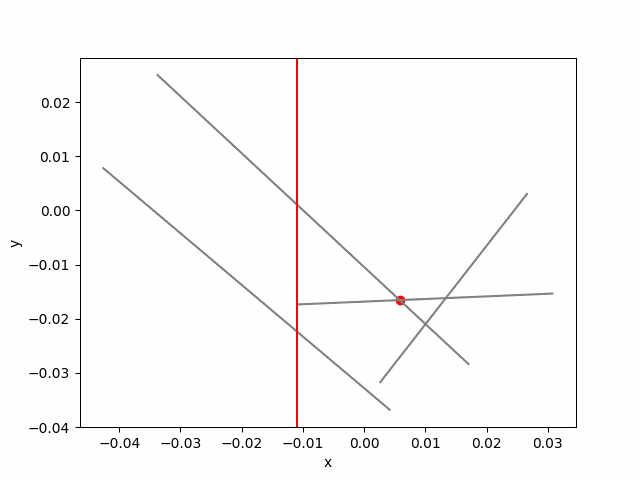
\includegraphics[width=\linewidth]{images/wyn1.png}
		\caption*{Rys. 7}
	\end{subfigure}
	\hfill
	\begin{subfigure}[t]{.45\textwidth}
		\centering
		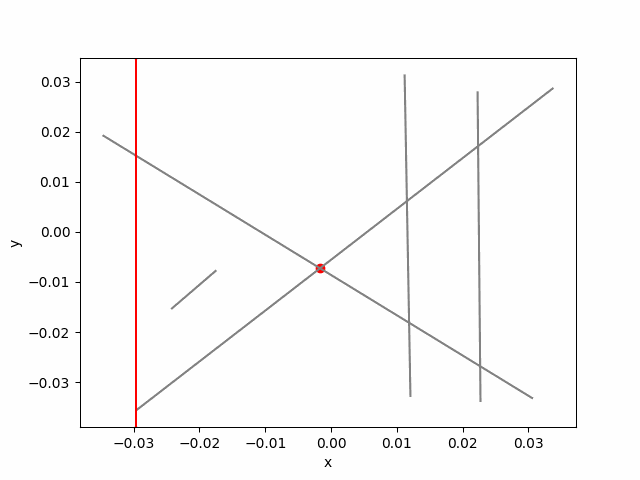
\includegraphics[width=\linewidth]{images/wyn2.png}
		\caption*{Rys. 8}
	\end{subfigure}
\end{figure}
\begin{figure}[htp]
	\begin{subfigure}[t]{.45\textwidth}
		\centering
		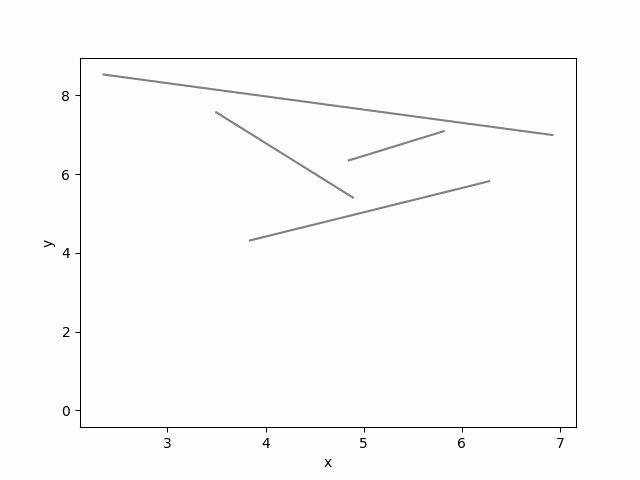
\includegraphics[width=\linewidth]{images/wyn6.png}
		\caption*{Rys. 9}
	\end{subfigure}
	\hfill
	\begin{subfigure}[t]{.45\textwidth}
		\centering
		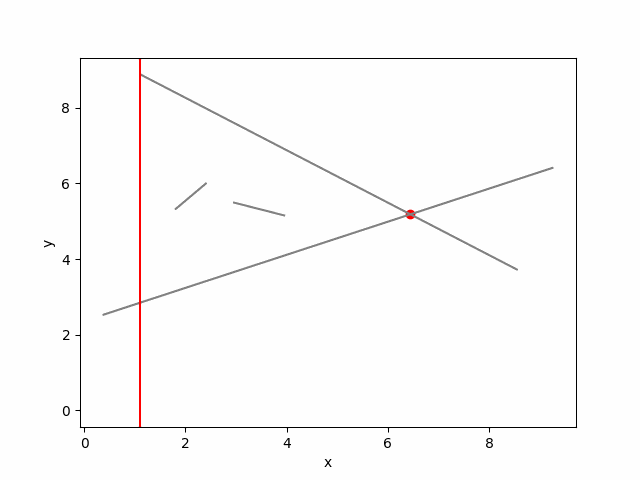
\includegraphics[width=\linewidth]{images/wyn7.png}
		\caption*{Rys. 10}
	\end{subfigure}
\end{figure}

\newpage
\section*{Implementacja rozwiązania}
\begin{Verbatim}
def is_intersection(sections):
	lines = create_lines(sections)
	T = SortedList()  # strukturę stanu T
	Q = SortedSet()  # struktura zdarzeń Q
	Line.brush_x = None
	for line in lines:
		Q.add(line.l_point)
		Q.add(line.r_point)
	while Q:
		p = Q.pop(0)
		left_neighbour_index = None  # porównaj z następnym odcinkiem
		right_neighbour_index = None  # porónaj z poprzednim odcinkiem
		# zaktualizuj T
		if p.type == -1:  # dodaj odcinek do T
			line = p.lines.pop()
			T.add(line)
			right_neighbour_index = T.bisect_right(line)
			left_neighbour_index = right_neighbour_index - 2
		elif p.type == 1:  # usuń odcinek z T
			line = p.lines.pop()
			T.remove(line)
			right_neighbour_index = T.bisect_right(line)
			left_neighbour_index = right_neighbour_index - 1
		# zaktualizuj Q
		new_intersections = set()
		if left_neighbour_index >= 0 and left_neighbour_index + 1 < len(T):
			new_intersections.add(lines_intersection(T[left_neighbour_index], 
			T[left_neighbour_index + 1]))
		if left_neighbour_index + 1 != right_neighbour_index 
		and right_neighbour_index - 1 >= 0 and right_neighbour_index < len(T):
			new_intersections.add(lines_intersection(T[right_neighbour_index - 1], 
			T[right_neighbour_index]))
		new_intersections.discard(None)
		for new_intersection in new_intersections:
			if new_intersection not in Q and new_intersection.x > Line.brush_x:
				return True
	return False
\end{Verbatim}

\newpage

\section*{Znajdowanie wszystkich przecięć odcinków}
Utwórz pustą strukturę stanu T

Utwórz strukturę zdarzeń Q – wstaw posortowane wzdłuż x końce odcinków

Powtarzaj

\quad ◦ pobierz nowe zdarzenie p z Q

\quad ◦ zaktualizuj T:

\quad \quad • jeśli p jest lewym końcem odcinka – dodaj odcinek do T

\quad \quad • jeśli p jest prawym końcem odcinka – usuń odcinek z T

\quad \quad • jeśli p jest punktem przecięcia s i s’, zmień porządek s i s’ w T

\quad ◦ zaktualizuj Q:

\quad \quad • dla każdej pary nowych sąsiadów s i s’ z T sprawdź, czy s i s’ przecinają się 

\quad \quad po prawej stronie miotły jeśli tak – dodaj punkt przecięcia do Q

\quad \quad • usuń możliwe duplikaty z Q

aż Q będzie puste

\section*{Wizualizacja wyników}
\begin{figure}[htp]
	\begin{subfigure}[t]{.45\textwidth}
		\centering
		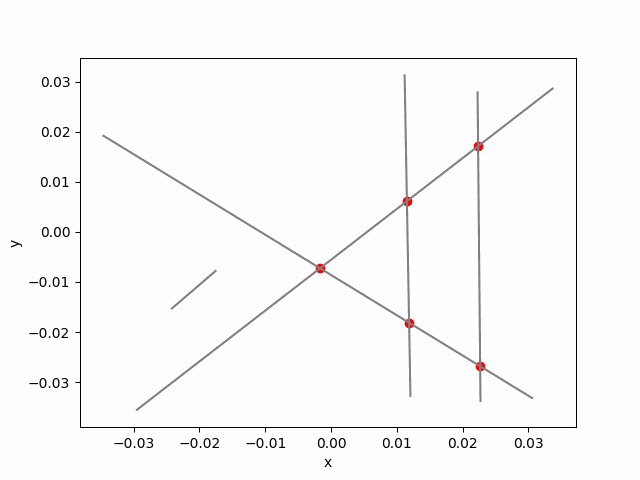
\includegraphics[width=\linewidth]{images/wyn3.png}
		\caption*{Rys. 11}
	\end{subfigure}
	\hfill
	\begin{subfigure}[t]{.45\textwidth}
		\centering
		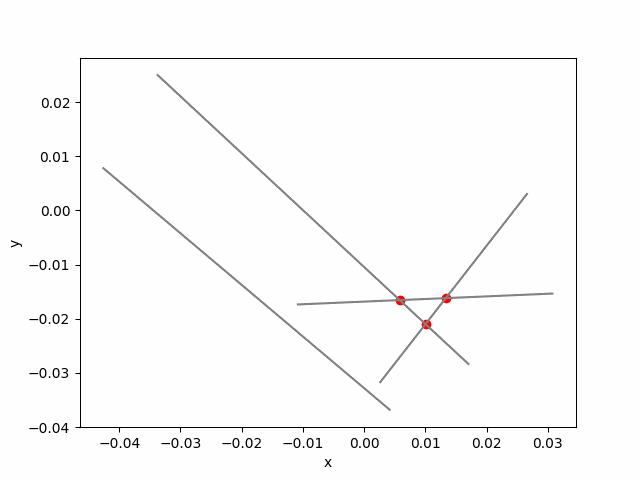
\includegraphics[width=\linewidth]{images/wyn4.png}
		\caption*{Rys. 12}
	\end{subfigure}
\end{figure}

\begin{figure}[htp]
	\begin{subfigure}[t]{.45\textwidth}
		\centering
		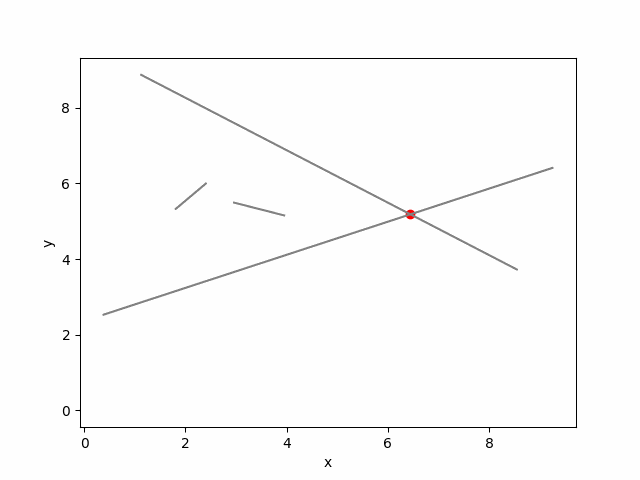
\includegraphics[width=\linewidth]{images/wyn5.png}
		\caption*{Rys. 13}
	\end{subfigure}
	\hfill
	\begin{subfigure}[t]{.45\textwidth}
		\centering
		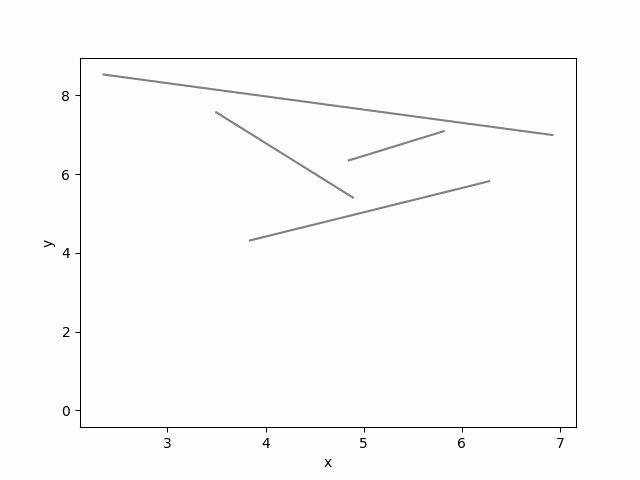
\includegraphics[width=\linewidth]{images/wyn6.png}
		\caption*{Rys. 14}
	\end{subfigure}
\end{figure}


\newpage
\section*{Implementacja rozwiązania}
\begin{Verbatim}
def find_intersections(sections):
	result = []
	lines = create_lines(sections)
	
	T = SortedList()  # strukturę stanu T
	Q = SortedSet()  # struktura zdarzeń Q
	Line.brush_x = None
	for line in lines:
		Q.add(line.l_point)
		Q.add(line.r_point)
	
	while Q:
		p = Q.pop(0)
		Line.brush_x = p.x
		left_neighbour_index = None  # porównaj z następnym odcinkiem
		right_neighbour_index = None  # porónaj z poprzednim odcinkiem
		
		# zaktualizuj T
		if p.type == -1:  # dodaj odcinek do T
			line = p.lines.pop()
			T.add(line)
			right_neighbour_index = T.bisect_right(line)
			left_neighbour_index = right_neighbour_index - 2
		
		elif p.type == 1:  # usuń odcinek z T
			line = p.lines.pop()
			T.remove(line)
			right_neighbour_index = T.bisect_right(line)
			left_neighbour_index = right_neighbour_index - 1
		
		elif p.type == 0:  # zmień porządek s i s’ w T
			line1 = p.lines.pop()
			line2 = p.lines.pop()
			Line.brush_x -= Point.EPSILON
			T.remove(line1)
			T.remove(line2)
			Line.brush_x += 2 * Point.EPSILON
			T.add(line1)
			T.add(line2)
			right_neighbour_index = max(T.bisect_right(line1), 
				T.bisect_right(line2))
			left_neighbour_index = right_neighbour_index - 3
vvvvvvvvvvvvvvvvvvvvvvvvvvvvvvvvvvvvvvvvvvvvvvvvvvvvvvvvvvvvvvvvvvvvvvvvvvvvvvvv
\end{Verbatim}
\newpage
\begin{Verbatim}
^^^^^^^^^^^^^^^^^^^^^^^^^^^^^^^^^^^^^^^^^^^^^^^^^^^^^^^^^^^^^^^^^^^^^^^^^^^^^^^^
		# zaktualizuj Q
		new_intersections = set()
		if left_neighbour_index >= 0 and left_neighbour_index + 1 < len(T):
			new_intersections.add(lines_intersection(T[left_neighbour_index], 
				T[left_neighbour_index + 1]))
		if left_neighbour_index + 1 != right_neighbour_index 
			and right_neighbour_index - 1 >= 0 and right_neighbour_index < len(T):
			new_intersections.add(lines_intersection(T[right_neighbour_index - 1],
				T[right_neighbour_index]))
		new_intersections.discard(None)
		for new_intersection in new_intersections:
			if new_intersection not in Q and new_intersection.x > Line.brush_x:
				Q.add(new_intersection)
				result.append((new_intersection.as_tuple(), 
					list(new_intersection.lines)[0].id + 1, 
					list(new_intersection.lines)[1].id + 1))

	return result
\end{Verbatim}

		\section*{Wnioski:}
		\begin{itemize}
			\item Analizując wyniki, oba algorytmy znalazły poprawne rozwiązania.
			\item Wymagana modyfikacja stanu pomiędzy problemem znajdowania dowolnego przecięcia, a wszystkich przecięć polega na dodawaniu wcześniej znalezionych punktów przecięcia, aby uwzględnić nowych sąsiadów po zamianie kolejności odcinków w T.
			\item Dobrana struktura zdarzeń Q zapobiega duplikowaniu się odcinków (np. Rys 13)
			\item Złożoność obliczeniowa naszego algorytmu wynosi \verb|O((P+n) log n)|, gdzie \verb|P| to liczba przecięć, czyli jest lepsza od podejścia w którym sprawdzamy wszystkie pary odcinków w czasie \verb|O(n^2)|.

		\end{itemize}
		
		
		
		
		
	\end{document}
